% \iffalse meta-comment
%
% Copyright (C) 2021 by Philippe Faist, philippe.faist@bluewin.ch
% -------------------------------------------------------
% 
% This file may be distributed and/or modified under the
% conditions of the LaTeX Project Public License, either version 1.3
% of this license or (at your option) any later version.
% The latest version of this license is in:
%
%    http://www.latex-project.org/lppl.txt
%
% and version 1.3 or later is part of all distributions of LaTeX 
% version 2005/12/01 or later.
%
% \fi
%
% \iffalse
%<*driver>
\ProvidesFile{phflplx.dtx}
%</driver>
%<package>\NeedsTeXFormat{LaTeX2e}[2005/12/01]
%<package>\ProvidesPackage{phflplx}
%<*package>
    [2021/04/09 v0.1 phflplx package]
%</package>
%
%<*driver>
\documentclass{ltxdoc}
\usepackage{xcolor}
\usepackage{lipsum}
\usepackage[preset=xpkgdoc]{phfnote}
\usepackage{phflplx}
\DeclareGraphicsExtensions{.lplx,.pdf}

\usepackage{needspace}

\def\eqsign@{=}
\def\eqsign{\protect\eqsign@}
\robustify\eqsign
\makeatother

\EnableCrossrefs
\CodelineIndex
\RecordChanges

\begin{document}
  \DocInput{phflplx.dtx}
\end{document}
%</driver>
% \fi
%
% \CheckSum{0}
%
% \CharacterTable
%  {Upper-case    \A\B\C\D\E\F\G\H\I\J\K\L\M\N\O\P\Q\R\S\T\U\V\W\X\Y\Z
%   Lower-case    \a\b\c\d\e\f\g\h\i\j\k\l\m\n\o\p\q\r\s\t\u\v\w\x\y\z
%   Digits        \0\1\2\3\4\5\6\7\8\9
%   Exclamation   \!     Double quote  \"     Hash (number) \#
%   Dollar        \$     Percent       \%     Ampersand     \&
%   Acute accent  \'     Left paren    \(     Right paren   \)
%   Asterisk      \*     Plus          \+     Comma         \,
%   Minus         \-     Point         \.     Solidus       \/
%   Colon         \:     Semicolon     \;     Less than     \<
%   Equals        \=     Greater than  \>     Question mark \?
%   Commercial at \@     Left bracket  \[     Backslash     \\
%   Right bracket \]     Circumflex    \^     Underscore    \_
%   Grave accent  \`     Left brace    \{     Vertical bar  \|
%   Right brace   \}     Tilde         \~}
%
%
% \changes{v0.1}{2021/04/09}{Initial version}
%
% \GetFileInfo{phflplx.dtx}
%
% \iffalse Bypass indexing for following commands: \fi
% \DoNotIndex{\newcommand,\newenvironment,\renewcommand,\long,\def,\edef,\gdef,\xdef,\if,\else,\fi,\par,\relax,\vspace,\vskip,\hspace,\hskip,\vbox,\hbox}
% 
% \title{The \pkgname{phflplx} package --- include PDF graphics with hyperlinks}
% \author{Philippe Faist\quad\email{philippe.faist@bluewin.ch}}
% \date{\pkgfmtdate\filedate}
% \maketitle
%
% \begin{abstract}
%   \pkgname{phflplx}---A handy \LaTeX{} package for including graphics defined
%   via \LaTeX\ source code files.  Designed for use with the |ltxpdflinks| tool
%   in order to include PDF graphics in documents with external or internal
%   hyperlinks.
% \end{abstract}
%
% \phantomsection\label{sec:toc}
% \inlinetoc
%
% \section{Introduction}
% \label{sec:intro}
%
% This package is designed to be used in conjunction with the |ltxpdflinks|
% command-line utility to extract PDF links into |.lplx| files.
%
% Usage:
%
% \begin{enumerate}[label=\arabic*.]
% \item Run |ltxpdflinks| on your PDF files before you compile your document:
% \begin{verbatim}
% > ltxpdflinks myfigure.pdf
% \end{verbatim}
%
% \item Use the following commands in your document preamble:
% \begin{verbatim}
% \usepackage{phflplx}
% \DeclareGraphicsExtensions{.lplx,.pdf}
% \end{verbatim}
%
% \item Drop a copy of |phflplx.sty| in the same folder as your document in case
%   you don't have it installed user-wide or system-wide.
%
% \item Enjoy!
% \end{enumerate}
% 
%
% In fact, LPLX files are simple LaTeX sources that are included directly by the
% graphics driver.  The LPLX file typically includes the PDF itself using a
% lower-level graphics command and draws invisible hyperlinks on top of the
% graphics.  (The LPLX file also takes care of resizing and cropping the
% graphics if necessary.)
%
% Figure~\ref{fig:Test} provides a glimpse of what you can do with |ltxpdflinks|
% and \pkgname{phflplx}.
% \begin{figure}
%   \centering
%   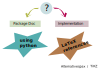
\includegraphics{diagram}
%   \caption{A diagram with clickable PDF hyperlinks, including internal links
%   to other parts of the document.}
%   \label{fig:Test}
% \end{figure}
%
%
% \section{Using the \phfverb{ltxpdflinks} script}
%
% Use the |ltxpdflinks| python script (|pip install ltxpdflinks|) to process
% your PDF files and generate an accompanying LPLX file.  The LPLX file is then
% picked up and links are rendered accordingly.
%
% The |ltxpdflinks| script will understand the following type of links:
%
% \begin{itemize}
% \item |https://example.com/| --- Regular URLs generate a web link to the given
%   location, as expected.
%
% \item |latexref://ref/<anchor>| and |latexref://cite/<citekey>| --- Special
%   URLs with the fictitious |latexref://| scheme are treated as internal LaTeX
%   references and citations (|ref| or |cite| fictitious domain).  The
%   |<anchor>| and |<citekey>| are arguments that you would provide to |\ref| or
%   |\cite|, respectively.
%
% \item |latexbox://<boxdomain>/<boxname>|, optionally
%   |latexbox://<boxdomain>/<boxname>?<key1>=<value1>&<key2>=<value2>...| ---
%   Special URLs with the fictitious |latexbox://| protocol are treated as an
%   instruction to look up data provided from the LaTeX document and include it
%   in the figure.  You can use this to include math, custom references, or any
%   LaTeX content you'd like to add in the figure.
%
%   The |<boxdomain>| and |<boxname>| refer to a named ``box'' defined using the
%   |\phflplxDefineBox| command (below).
%
%   You can specify the additional arguments as standard URL query string
%   arguments:
%   \begin{itemize}
%   \item |valign=...| How to align the content vertically.  One of |t| (top),
%     |c| (center), or |b| (bottom).
%   \item |halign=...| How to align and typeset the content horizontally.  One
%     of |l| (left), |c| (center), |r| (right), |p| (just typeset the paragraph
%     normally w/o additional alignment commands), |ml| (left on one line, using
%     a |\makebox|), |mc| (center on one line, using a |\makebox|), |mr| (right
%     on one line, using a |\makebox|), or |ms| (spread on one line, using a
%     |\makebox|).
%   \item |stylemacro=macroname| Wrap the contents within a call to the given
%     styling macro (name without the backslash).  Use for instance
%     |stylemacro=textbf| to typeset the content in boldface font.
%   \end{itemize}
% \end{itemize}
%
%
% \DescribeMacro{\phflplxDefineBox} To provide content from the LaTeX document
% that the figure can include via a |latexbox://|-type url, use the
% |\phflplxDefineBox| macro:
%
% |\phflplxDefineBox|\marg{boxdomain}\marg{boxname}\marg{content}
%
% The \meta{boxdomain} and \meta{boxname} are your user-defined keys.  We
% suggest having |boxdomain| matching the name of the figure and |boxname| to be
% a meaningful name describing the content you're saving.  The \meta{content}
% can be arbitrary content that will be placed where the figure requested the
% given box.
%
%
% \StopEventually{\PrintChangesAndIndex}
%
% \section{Implementation}
% \label{sec:implementation}
%
% Load some useful packages.
%    \begin{macrocode}
\RequirePackage{etoolbox}
%    \end{macrocode}
%
% Check that the user is loading the \pkgname{hyperref} package! (We don't load
% it automatically to avoid issues of package loading order, link appearance,
% etc.)
%    \begin{macrocode}
\AtBeginDocument{%
  \@ifpackageloaded{hyperref}{}{%
    \PackageWarning{phflplx}{The package `hyperref' was not loaded. You
      probably forgot to load it.}%
  }%
}
%    \end{macrocode}
%
%
% \subsection{Integration into graphics/graphicx package}
% 
% Declaring the graphics rule for the LPLX extension.  Note that the LPLX file
% has the line |%%BoundingBox 0 0 <W> <H>| so that the size of the graphics can
% be parsed by the default \pkgname{graphics} graphic size inspector, which is
% designed to parse |%%BoundingBox| commands in EPS files.
%    \begin{macrocode}
\DeclareGraphicsRule{.lplx}{lplx}{*}{}
%    \end{macrocode}
% 
% Declare the driver functions for the \pkgname{graphics} package internals.
%    \begin{macrocode}
\def\Ginclude@lplx#1{%
  \message{<#1>}%
  \input{#1}%
}
%    \end{macrocode}
%
%
% \subsection{Commands called from the LPLX file}
%
% The contents of the LPLX file is wrapped around the |\LPLX| macro.  The first
% argument is a dictionary |key1=value1,key2=value2,...| of meta-information
% about the current LPLX file format.  Keys should include |version| (a basic
% file format version), |ltxpdflinksversion| (version of |ltxpdflinks| used to
% generate this file), |features| (a list of ``features'' the file provides,
% might add new ``features'' in the future).  The ``|bbox|'' feature means that
% the LPLX file makes a call to |\lplxSetBbox| with the graphic bounding box
% information.
%    \begin{macrocode}
%%\long\def\LPLX#1#2{\begingroup #2\endgroup}
\let\LPLX\@gobble
%    \end{macrocode}
%
% In the contents of the LPLX data (second argument of |\LPLX|), we have a
% sequence of |\lplxAbcDef| commands in a declarative-style interface.
% The commands are the following.
%
% \begin{macro}{\lplxGraphic}
%   Specify the original (PDF) graphic file name.  Specify base file name (|#1|)
%   and extension (|#2| including dot) separately
%    \begin{macrocode}
\def\lplxGraphic#1#2{%
  \def\lplxiGraphicBaseFname{#1}%
  \def\lplxiGraphicExt{#2}%
  \def\lplxiGraphicFname{#1#2}%
  \lplx@IncludeGraphics
}
%    \end{macrocode}
% \end{macro}
%
% \begin{macro}{\lplxUserSpaceUnitLength}
%   Set the base unit of the graphic.  Width, height, coordinates, etc., are
%   specified in this unit.  Usually this is $1\textrm{ bp} = 1/72\textrm{ in}$.
%    \begin{macrocode}
\def\lplxUserSpaceUnitLength#1{%
  \unitlength=#1\relax
}
%    \end{macrocode}
% \end{macro}
%
% \begin{macro}{\lplxSetBbox}
%   Declare what the bounding box of the graphic is.  Currently the two first
%   arguments should be |{0}{0}|.
%    \begin{macrocode}
\newdimen\lplxiBboxWcrdim
\newdimen\lplxiBboxHcrdim
\def\lplxSetBbox#1#2#3#4{%
  \def\lplxiBboxX{#1}%
  \def\lplxiBboxY{#2}%
  \def\lplxiBboxW{#3}%
  \def\lplxiBboxH{#4}%
  \ifdim\lplxiBboxX\p@>\z@\relax\lplx@bboxzerowarn\fi
  \ifdim\lplxiBboxX\p@<\z@\relax\lplx@bboxzerowarn\fi
  \ifdim\lplxiBboxY\p@>\z@\relax\lplx@bboxzerowarn\fi
  \ifdim\lplxiBboxY\p@<\z@\relax\lplx@bboxzerowarn\fi
}
\def\lplx@bboxzerowarn{%
  \PackageWarning{phflplx}{LPLX bounding box is not pinned at (0,0), not supported}%
}
%    \end{macrocode}
% \end{macro}
%
% \begin{macro}{\lplxPicture}
%   Gather all the links you want to place as an argument to a call to
%   |\lplxPicture|.
%    \begin{macrocode}
\long\def\lplxPicture#1{%
  \lplx@SetupScaleAndBbox
  \lplx@a@DoScale{%
    \begin{picture}(\lplxvCropW,\lplxvCropH)(\lplxvCropX,\lplxvCropY)%
      #1%
    \end{picture}%
  }%
}
%    \end{macrocode}
% \end{macro}
% 
% Finally, individual links are placed with |\lplxPutLink|.  Usage is
% |\lplxPutLink|\marg{x}\marg{y}\marg{w}\marg{h}\marg{hyperstartcmd}\marg{hyperendtokens}.
% Here \marg{hyperstartcmd} and \marg{hyperendtokens} are any tokens that will
% be inserted immediately before and immediately after an invisible rule of the
% given width and height.  The rule will be in curly braces, so it can be
% considered as a mandatory argument to the last macro token in
% \marg{hyperstartcmd}.  Don't forget to escape URL characters that have a LaTeX
% meaning that is very special (e.g. |#| $\to$
% |%23|) because these characters are already in a macro argument and
% will have catcodes assigned before |\href| and friends get the chance to take
% care of catcodes etc.  [Actually, some characters still work, like |^|, |_|,
% |&|, \ldots\space  I'm not sure what determines this. (?)]
%    \begin{macrocode}
\def\lplxPutLink{%
  \ifGin@clip
    \expandafter\lplx@clipputlink
  \else
    \expandafter\lplx@doputlink
  \fi
}
%    \end{macrocode}
%
% Helper to place other content than a link, using the |\lplxPutLink| mechanism
% (for placing latex boxes).  The |\@gobble| simply gobbles the default
% invisible rectangular box that is supposed to be the hyperlink's content.
%    \begin{macrocode}
\def\lplxPlaceContent#1#2#3#4#5{% x,y,w,h,content
  \lplxPutLink{#1}{#2}{#3}{#4}{\@gobble}{#5}%
}
%    \end{macrocode}
% 
% A simple helper to percent-quote special characters in an URL.
%
%    \begin{macrocode}
{\catcode`\%=12\relax
  \gdef\lplx@percent{%}
}
\def\lplxHexChar#1{%
  \lplx@percent#1%
}
%    \end{macrocode}
% 
%
% \subsection{Providing content to the figure from LaTeX --- ``placing boxes''}
%
% Special links in the PDF figure of the form
% |latexbox://<domain>/<boxname>?<arguments>| allow you to place custom content
% in the figure from LaTeX.  You can define that content using the
% |\phflplxDefineBox| command:
% \begin{macro}{\phflplxDefineBox}
%    \begin{macrocode}
\long\def\phflplxDefineBox#1#2#3{%
  \expandafter\gdef\csname lplx@def@box@#1@#2\endcsname{#3}%
}
%    \end{macrocode}
% \end{macro}
%
%
% Internal command that will be used to render the box from the generated LPLX
% code:
%    \begin{macrocode}
\long\def\lplx@render@box@set@halign@p#1{#1}
\long\def\lplx@render@box@set@halign@l#1{%
  \raggedright#1}
\long\def\lplx@render@box@set@halign@c#1{%
  \centering#1}
\long\def\lplx@render@box@set@halign@r#1{%
  \raggedleft#1}
\def\lplx@render@box@set@halign@ml{\makebox[\hsize][l]}
\def\lplx@render@box@set@halign@mc{\makebox[\hsize][c]}
\def\lplx@render@box@set@halign@mr{\makebox[\hsize][r]}
\def\lplx@render@box@set@halign@ms{\makebox[\hsize][s]}
\def\lplxRenderBox[#1]#2[#3]#4#5#6#7{% halign,w,valign,h,stylemacro,boxdomain,boxname
%%  \message{***LPLX BOX *** |\detokenize{#1}| |\detokenize{#2}| |\detokenize{#3}| |\detokenize{#4}| |\detokenize{#5}| |\detokenize{#6}|}%
  \parbox[b][#4][#3]{#2}{%
    \vsize=#4\relax
    \csname lplx@render@box@set@halign@#1\endcsname
    {#5{\lplx@render@box@contents{#6}{#7}}}%
  }%
}
\def\lplx@render@box@contents#1#2{%
  \csname lplx@def@box@#1@#2\endcsname
}
%    \end{macrocode}
%
% \subsection{Internal Implementation Commands}
%
%
%
% \begin{macro}{\lplx@IncludeGraphics}
%   This command actually includes the underlying graphics.  TODO: support for
%   |\lplxiGraphicFname| in case the PDF base file name differs from the LPLX
%   file base name? (Though that sounds like asking for trouble.)
%    \begin{macrocode}
\def\lplx@IncludeGraphics{%
  \edef\x{\noexpand\hbox to 0pt{%
      \noexpand\Ginclude@graphics{\Gin@base\lplxiGraphicExt}}}%
  \x
}
%    \end{macrocode}
% \end{macro}
% 
% \begin{macro}{\lplx@SetupScaleAndBbox}
%   Utility to set up the appropriate command arguments to use for |\scalebox|,
%   etc.
%    \begin{macrocode}
\def\lplx@noscale{1,!}
\def\lplx@exclam{!}
\def\lplx@a@DoScale{}%
\def\lplx@SetupScaleAndBbox{%
%    \end{macrocode}
% 
% First, we locally define a macro |\lplx@a@DoScale{...}| that will generate the
% correct |\scalebox| call with the given contents, according to the requested
% size.
%    \begin{macrocode}
  \def\lplx@tmp{\Gin@scalex,\Gin@scaley}%
  \ifx\lplx@tmp\lplx@noscale%
    \def\lplx@a@DoScale{}%
  \else
    \ifx\Gin@scaley\lplx@exclam
      \edef\lplx@a@DoScale{\noexpand\scalebox{\Gin@scalex}}%
    \else
      \ifx\Gin@scalex\lplx@exclam
        \edef\lplx@a@DoScale{\noexpand\scalebox{\Gin@scaley}}%
      \else
        \edef\lplx@a@DoScale{\noexpand\scalebox{\Gin@scalex}[\Gin@scaley]}%
      \fi
    \fi
  \fi
%    \end{macrocode}
% Second, we need to take care of setting the bounding box correctly.  Define
% the macros |\lplxvCropX| and |\lplxvCropY| which are the $(X,Y)$ position of
% the lower left corner the part of the image we want to pick out, in user space
% units.  Define |\lplxvCropW| and |\lplxvCropH| as the requested width \&
% height of the subimage we want to use.
%    \begin{macrocode}
  \edef\lplxvCropX{\Gin@llx}%
  \edef\lplxvCropY{\Gin@lly}%
  \edef\lplxvCropW{\strip@pt\dimexpr\Gin@urx pt-\Gin@llx pt\relax}%
  \edef\lplxvCropH{\strip@pt\dimexpr\Gin@ury pt-\Gin@lly pt\relax}%
}
%    \end{macrocode}
% \end{macro}
%
%
% Tools to place links \& clip them if necessary.
%    \begin{macrocode}
\def\lplx@phantomrule#1#2{% w, h (dimensions given as the string "Xbp")
  {\phantom{\rule{#1}{#2}}}%
}
\def\lplx@doputlink#1#2#3#4#5#6{% x,y,w,h,hyperstart,hyperend
  \put(#1,#2){#5{\lplx@phantomrule{#3bp}{#4bp}}#6}%
}%
\newdimen\lplx@tmpx
\newdimen\lplx@tmpy
\newdimen\lplx@tmpw
\newdimen\lplx@tmph
\def\lplx@clipputlink#1#2#3#4#5#6{% x,y,w,h,hyperstart,hyperend
%    \end{macrocode}
% Some notes: 1) We use ``pt'' as dummy unit of measure here just to do the
% floating point arithmetic and we use |\strip@pt| at the end.  2) Here
% |\lplx@maybeskip| serves as a flag that if set, asserts the link was entirely
% cropped out of the picture.  Initially it expands to an empty string but when
% set it expands to ``|\p@<\z@\relax|'' (= ``|1pt < 0pt|''), so it can be placed
% in front of all |\ifdim|'s so that they are skipped if the link was determined
% to be out of the picture.
%    \begin{macrocode}
  \def\lplx@maybeskip{}%
  \def\lplx@setskip{\def\lplx@maybeskip{\p@<\z@\relax}}%
  \lplx@tmpx=#1pt\relax
  \lplx@tmpy=#2pt\relax
  \lplx@tmpw=#3pt\relax
  \lplx@tmph=#4pt\relax
  \ifdim\lplx@maybeskip\lplx@tmpx<\lplxvCropX\p@\relax
    \ifdim\dimexpr\lplx@tmpx+\lplx@tmpw>\lplxvCropX\p@\relax
      \lplx@tmpw=\dimexpr\lplx@tmpx+\lplx@tmpw-\lplxvCropX\p@\relax
      \lplx@tmpx=\lplxvCropX\p@\relax
    \else
      \lplx@setskip
    \fi
  \fi
  \ifdim\lplx@maybeskip\dimexpr\lplx@tmpx+\lplx@tmpw
        >\dimexpr\lplxvCropX\p@+\lplxvCropW\p@\relax
    \ifdim\lplx@tmpx<\dimexpr\lplxvCropX\p@+\lplxvCropW\p@\relax
      \lplx@tmpw=\dimexpr\lplxvCropX\p@+\lplxvCropW\p@-\lplx@tmpx\relax
    \else
      \lplx@setskip
    \fi
  \fi
  \ifdim\lplx@maybeskip\lplx@tmpy<\lplxvCropY\p@\relax
    \ifdim\dimexpr\lplx@tmpy+\lplx@tmph>\lplxvCropY\p@\relax
      \lplx@tmph=\dimexpr\lplx@tmpy+\lplx@tmph-\lplxvCropY\p@\relax
      \lplx@tmpy=\lplxvCropY\p@\relax
    \else
      \lplx@setskip
    \fi
  \fi
  \ifdim\lplx@maybeskip\dimexpr\lplx@tmpy+\lplx@tmph
        >\dimexpr\lplxvCropY\p@+\lplxvCropH\p@\relax
    \ifdim\lplx@tmpy<\dimexpr\lplxvCropY\p@+\lplxvCropH\p@\relax
      \lplx@tmph=\dimexpr\lplxvCropY\p@+\lplxvCropH\p@-\lplx@tmpy\relax
    \else
      \lplx@setskip
    \fi
  \fi
  \ifdim\lplx@maybeskip\p@>\z@\relax
    \edef\x{\noexpand\lplx@doputlink%
      {\strip@pt\lplx@tmpx}{\strip@pt\lplx@tmpy}%
      {\strip@pt\lplx@tmpw}{\strip@pt\lplx@tmph}}%
    \x{#5}{#6}%
  \fi
}%

%    \end{macrocode}
% 
%\Finale
\endinput
